\subsection{\large{Разработка расчётной модели данных}}
\addcontentsline{toc}{subsection}

Расчётная модель данных в отличие от модели данных конкретной методики содержит гораздо большее количество информации.
Расчётная модель данных состоит из расчётных элементов. Ниже представлена общая диаграмма классов расчётной модели данных
(см. рис.\ref{pic:implementation__model-classes}).

\begin{figure}[H]
	\hspace*{-2.5 cm}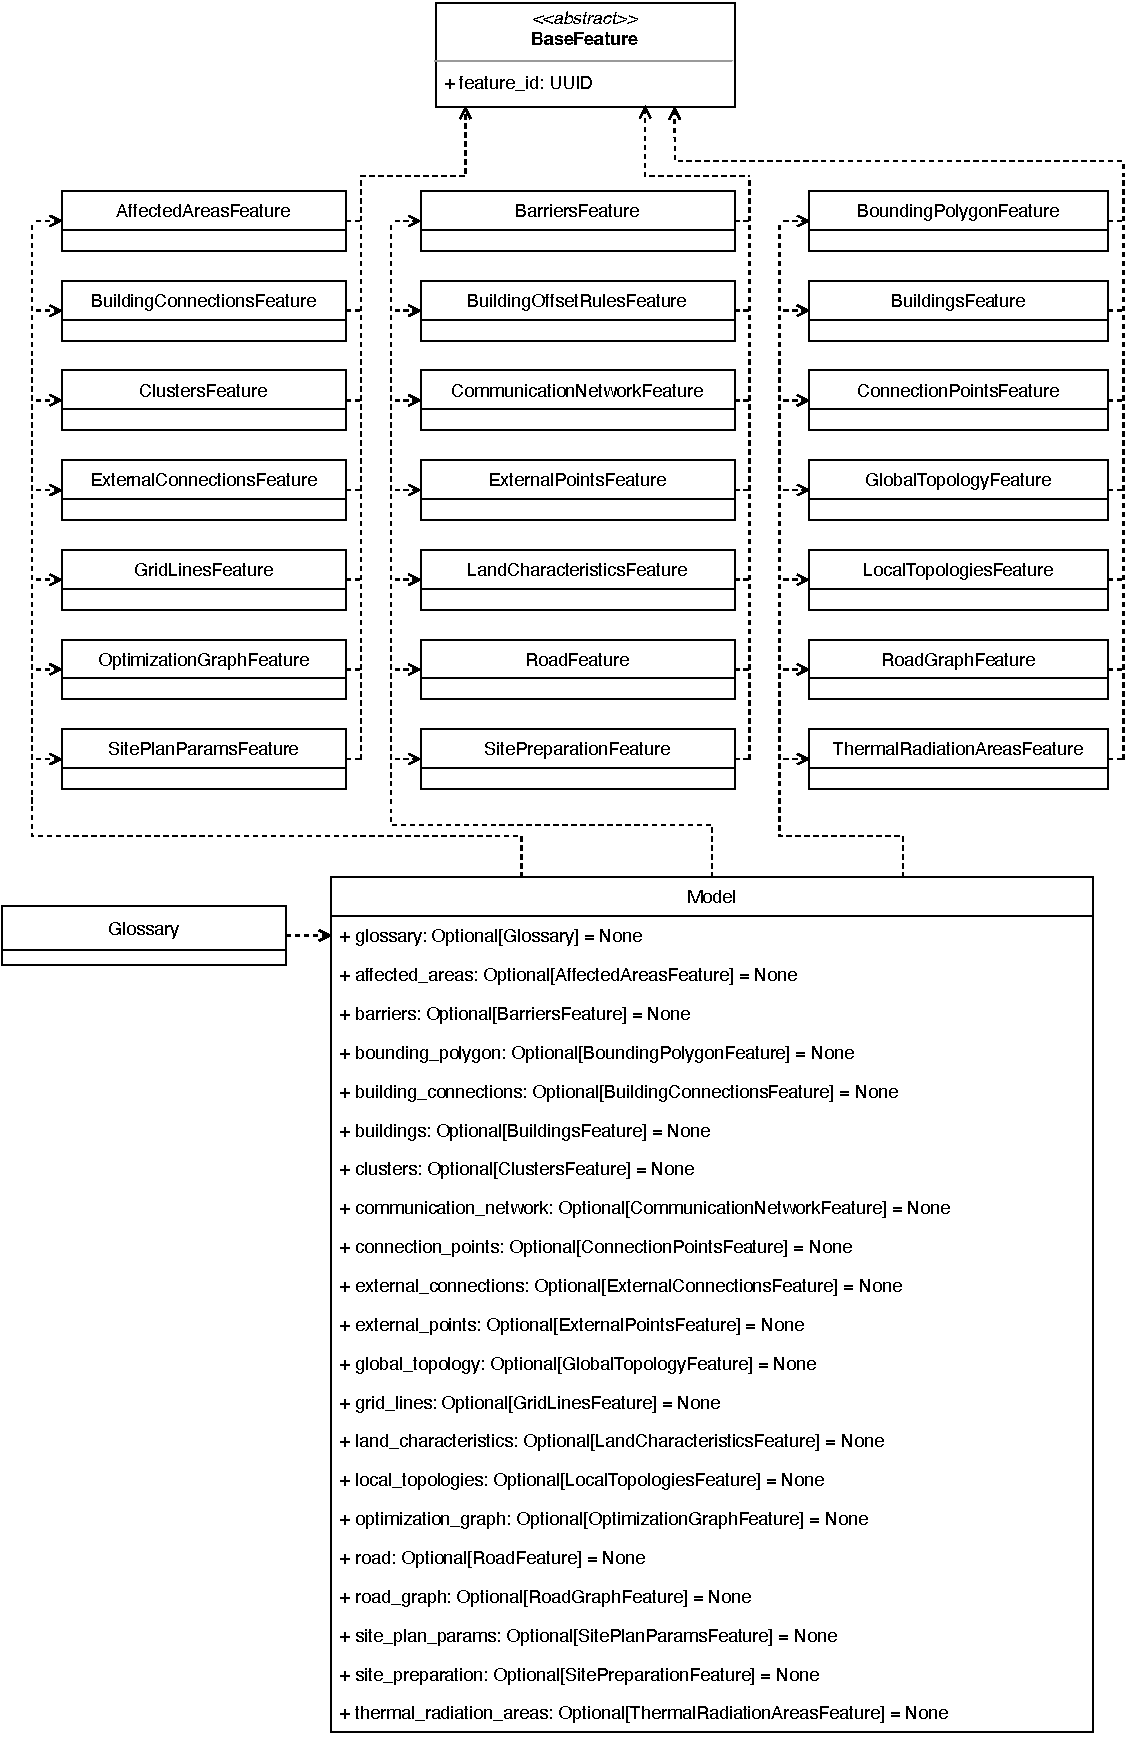
\includegraphics[width=0.7\textwidth]{implementation/pictures/model/classes}
	\caption{Общая диаграммма классов расчётной модели}
	\label{pic:implementation__model-classes}
\end{figure}
\vskip 5 mm

А вот диаграмма классов для расчётного элемента (см. рис.\ref{pic:implementation__model-feature}).
\begin{figure}[H]
	\hspace*{-2.5 cm}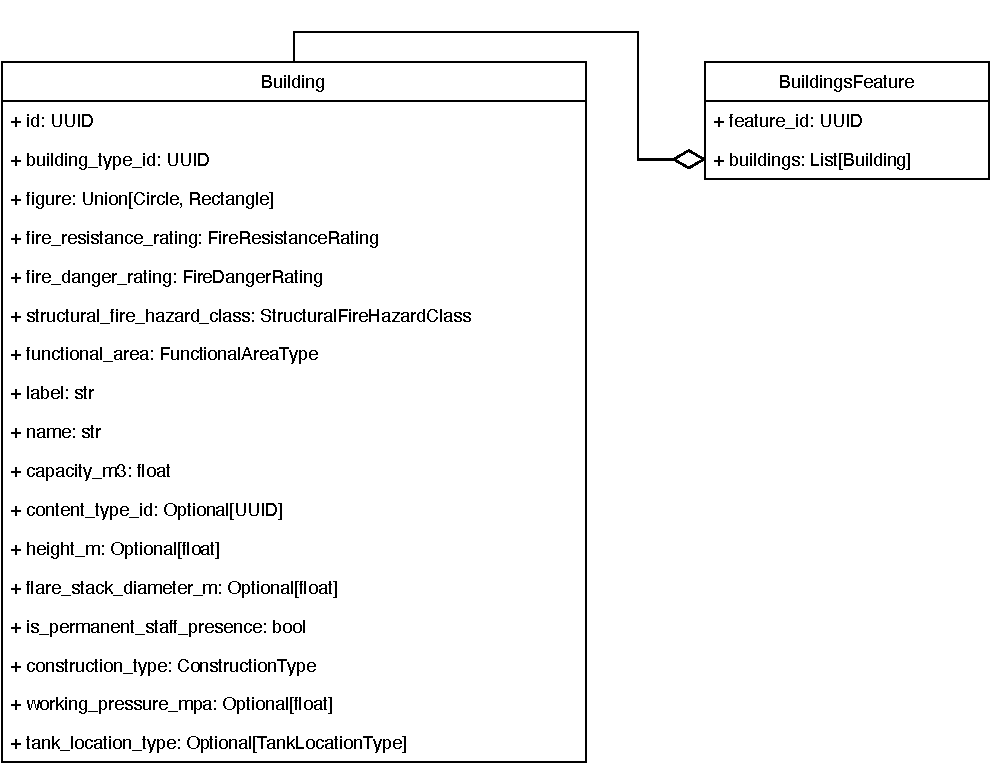
\includegraphics[width=0.7\textwidth]{implementation/pictures/model/feature}
	\caption{Общая диаграммма классов расчётной модели}
	\label{pic:implementation__model-feature}
\end{figure}
\vskip 5 mm

Класс \textit{Building} содержит 17 полей, а класс \textit{Flare}, описанного для методики расчёта
зон теплового излучения содержит всего 4 поля.
